\documentclass[a4paper,12pt]{article}
\usepackage[slovak]{babel}
\usepackage[utf8]{inputenc}
\usepackage{amsmath}
\usepackage[bookmarksopen,colorlinks,plainpages=false,urlcolor=blue]{hyperref}

\usepackage{ifpdf}

\ifpdf
  \usepackage[dvipdf]{graphicx}
\else
  \usepackage[dvips]{graphicx}
\fi

\usepackage[top=2cm, left=2cm, text={17cm, 26cm}, ignorefoot]{geometry}
\author{Patrik Holop - xholop01}

\begin{document}

\begin{figure}[!h]
  \centering
  
\includegraphics[height=5cm]{obrazky/fit}
\end{figure}

\begin{center}
\bigskip
\begin{Huge}
Elektronika pre informačné technológie\\
\bigskip
Semestrálny Projekt\\
2016/2017\\
\end{Huge}
\end{center}

\vfill

\begin{flushleft}
 \begin{large}
 Autor: Patrik Holop, ID 196279, xholop01@stud.fit.vutbr.cz\\
 Dátum: 11.12.2016
 \end{large}
\end{flushleft}

% End title page 
% --------------
% Start 1st 
\newpage
\begin{flushleft}
\textbf{1. príklad}\\
Varianta: C
\end{flushleft}

\begin{tabular}{|c|c|c|c|c|c|c|c|c|c|}
\hline $U_1$ & $U_2$ & $R_1$ & $R_2$ & $R_3$ & $R_4$ & $R_5$ & $R_6$ & $R_7$ & $R_8$ \\ 
\hline
$100V$ & $80V$ &  $450\Omega$ & $810\Omega$ & $190\Omega$ & $220\Omega$ & $220\Omega$ & $720\Omega$ & $260\Omega$ & $180\Omega$ \\ 
\hline
\end{tabular}
\bigskip

\begin{flushleft}
\textbf{Zadanie:}\\
Stanovte napětí $U_{R_8}$ a proud $I_{R_8}$. Použijte metodu postupného zjednodušování obvodu.
\end{flushleft}
\begin{flushleft}
\textbf{Postup:} \\ 
1. Obvod dokážeme postupne zjednodušovať \\
\end{flushleft}\begin{figure}[!h]
  \centering
  obr.1\\
  \bigskip
  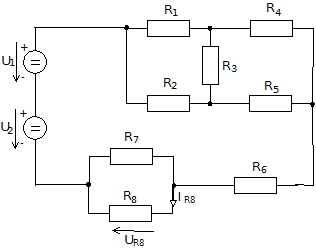
\includegraphics[height=5cm]{obrazky/pr1a} \\
  \bigskip
  obr.2
  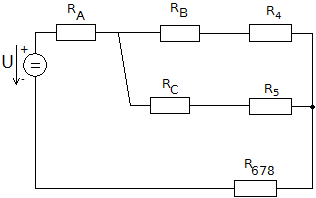
\includegraphics[height=4cm]{obrazky/pr1b} 
  obr.3
  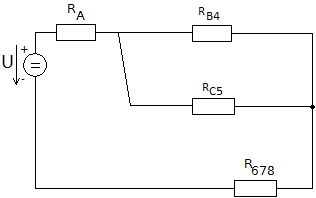
\includegraphics[height=4cm]{obrazky/pr1c} \\
  \bigskip
\end{figure}
\bigskip

\begin{flushleft}
Odpory $R_7$ a $R_8$ sú zapojené paralelne a toto spojenie je zapojené sériovo s odporom $R_6$. Nahradíme ich odporom $R_{678}$. Taktiež zdroje napätia $U_1$ a $U_2$ sú v sérii (a rovnakom smere), nahradíme ich napätím U.
\end{flushleft}
\begin{equation*}
obr.1 : R_{678} = \frac{R_{7}R_{8}}{R_7+R_8} + R_6
\end{equation*}
\begin{equation*}
U = U_1 + U_2
\end{equation*}

\begin{flushleft}
Zapojenie odporov $R_1$, $R_2$ a $R_3$ môžeme transformovať do zapojenia hviezdice a toto zapojenie nahradiť odpormi $R_A$, $R_B$, $R_C$. 
\end{flushleft}
\begin{equation*}
obr.2 : R_A = \frac{R_{1}R_{2}}{R_1+R_2+R_3} \quad R_B = \frac{R_{1}R_{3}}{R_1+R_2+R_3} 
\quad R_C = \frac{R_{2}R_{3}}{R_1+R_2+R_3} \\
\end{equation*}
\bigskip
\begin{flushleft}
Odpor $R_B$ a $R_4$ sú v sérii, ako aj $R_C$ a $R_5$. Obe tieto zapojenia sú navzájom zapojené paralelne a môžme ich nahradiť odporom $R_{B4C5}$.
\end{flushleft}
\begin{equation*}
obr.3 : R_{B4} = R_B + R_4 \quad R_{C5} = R_C + R_5 
\end{equation*}
\begin{equation*}
R_{B4C5} = \frac{R_{C5} * R_{B4}}{R_{C5} + R_{B4}}
\end{equation*}

\begin{flushleft}
Pretože sú $R_A$, $R_{B4C5}$ $R_{678}$ v sérii, môžeme zjednodušiť obvod na jednoduché zapojenie zdroja napätia a jedného odporu $R_{EKV}$:
\end{flushleft}
\begin{equation*}
R_{EKV} = R_A + R_{B4C5} + R_{678}
\end{equation*}

\begin{flushleft}
Dostávame zjednodušený obvod:
\end{flushleft}
\begin{figure}[!h]
  \centering
  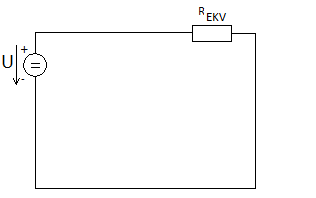
\includegraphics[height=4cm]{obrazky/pr1d}
\end{figure}

\begin{flushleft}
Po dosadení je výsledný vzorec ekvivalentného odporu v zjednodušenom obvode:
\end{flushleft}
\begin{equation*}
R_{EKV} = \frac{R_{1}R_{2}}{R_1+R_2+R_3}
+ \frac{(\frac{R_{1}R_{3}}{R_1+R_2+R_3}+R_4)(\frac{R_{2}R_{3}}{R_1+R_2+R_3}+R_5)}
       {\frac{R_{1} * R_{3}}{R_{1}+R_{2}+R_3} + R_4 + \frac{R_{2} * R_{3}}{R_{1}+R_{2}+R_3} + R_5  } 
+ R_6 + \frac{R_{7}R_{8}}{R_7+R_8} 
\end{equation*}

\begin{equation*}
R_{EKV} = 251,3793
+ \frac{(278,9655)(326,1379)}
       {278,9655 + 326,1379} 
+ 720 + 106,3636
\end{equation*}

\begin{equation*}
R_{EKV} = 1228,0995\Omega
\end{equation*}

\begin{flushleft}
Teraz môžeme vypočítať celkový prúd pretekajúci obvodom
\end{flushleft}

\begin{equation*}
I_{EKV} = \frac{U}{R_{EKV}}
\end{equation*}

\begin{equation*}
I_{EKV} = \frac{180}{1228,0995} = 0,1466 A
\end{equation*}

Vieme, že napätie $U_{R7}$ a $U_{R8}$ je rovnaké, pretože  $R_7$ a  $R_8$  sú zapojené paralelne. Ďalej vieme, že $I_{EKV}$ sa rozdelí do vetví na základe veľkostí odporov. 

\begin{equation*}
\frac{U_{R7}}{R_7} + \frac{U_{R8}}{R_8} = I_{EKV} \qquad U_{R7} = U_{R8}
\end{equation*}

\begin{equation*}
R_8*U_{R8} + R_7*U_{R8} = I_{EKV}*R_{8}*R_{7}
\end{equation*}

\begin{equation*}
U_{R8} = \frac{I_{EKV}*R_{8}*R_{7}}{R_7+R_8} =
= \frac{0,1466*180*260}{180+260} = 15,5895 V
\end{equation*}

\begin{equation*}
I_{R8} = \frac{U_{R8}}{R_8} = \frac{15,5895}{180} = 0,0866 A
\end{equation*}

% End 1st 
% --------------
% Start 2nd

\newpage
\begin{flushleft}
\textbf{2. príklad}\\
Varianta: H
\end{flushleft}

\begin{tabular}{|c|c|c|c|c|c|}
\hline $U_1$ & $R_1$ & $R_2$ & $R_3$ & $R_4$ & $R_5$ \\ 
\hline
$220V$ & $360\Omega$ & $580\Omega$ & $205\Omega$ & $560\Omega$ & $350\Omega$ \\ 
\hline
\end{tabular}
\bigskip

\begin{flushleft}
\textbf{Zadanie:}\\
Stanovte napětí $U_{R_4}$ a proud $I_{R_4}$. Použijte metodu Théveninovy věty.
\end{flushleft}
\begin{flushleft}
\textbf{Postup:} \\ 
1. Zadaný obvod (obr.1) vieme pomocou Theveninovej vety prepísať na náhradný obvod (obr.2) \\
\end{flushleft}
\begin{figure}[!h]
  \centering
  obr.1\\
  \bigskip
  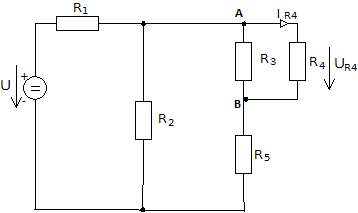
\includegraphics[height=5cm]{obrazky/pr2a} \\
  \bigskip
\end{figure}

\begin{figure}[!h]
  \centering
  obr.2\\
  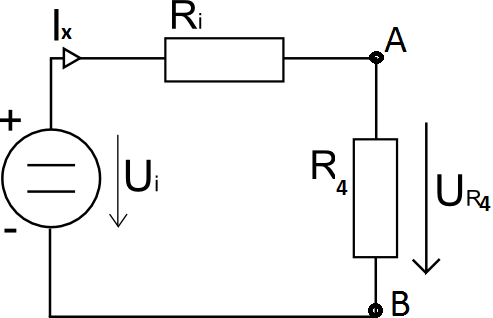
\includegraphics[height=4cm]{obrazky/pr2b}
\end{figure}
\begin{flushleft}
V náhradnom obvode sa celkový odpor rovná $R_i$ + $R_4$ a prechádza ním prúd $I_x$. Vypočítame $R_i$ (odpor medzi uzlami A a B)
\end{flushleft}
\begin{equation*}
R_{i} = \frac{(\frac{R_1R_2}{R_1+R_2} + R_5)*R_3}{\frac{R_1R_2}{R_1+R_2}+R_5+R_3} = \frac{117286,1702}{777,1277} = 150,9227\Omega
\end{equation*}

\begin{flushleft}
Na výpočet $U_i$ z náhradného obvodu budeme potrebovať prúdy prechádzajúce obvodom po skratovaní $R_4$. 
\end{flushleft}
\begin{equation*}
R_{EKV} = \frac{R_{2}*(R_3+R_5)}{R_3+R_5+R_2}+R_1 = 643,6123\Omega
\end{equation*}
\begin{equation*}
I_{R1} = \frac{U}{R_{EKV}} = 0,3442 A
\end{equation*}
\begin{equation*}
U_{R1} = R_1*I_{R1} = 123,0554 V
\end{equation*}
\begin{equation*}
U_{R2} = U-U_{R1} = 96,9446 V
\end{equation*}
\begin{equation*}
I_{R2} = \frac{U_{R2}}{R_2} = 0,1671 A
\end{equation*}
\begin{equation*}
I_{R3} = I_{R1} - I_{R2} = 0,1748 A
\end{equation*}

\bigskip
\begin{flushleft}
Teraz môžeme vypočítať $U_i$, napätie medzi uzlami A a B a $I_x$, prúd pretekajúci náhradným obvodom. Platí, že $U_i$ = $U_{R3}$.
\end{flushleft}
\begin{equation*}
U_i = R_3 * I_{R3} = 35,834 V
\end{equation*}
\begin{equation*}
I_x = \frac{U_i}{R_i+R_4} = \frac{35,834}{710,9227} = 0,0504 A
\end{equation*}
\begin{equation*}
I_x = I_{R4} \qquad U_{R4} = R_4*I_{R4} = 28,224 V
\end{equation*}

% End 2nd 
% --------------
% Start 3rd

\newpage
\begin{flushleft}
\textbf{3. príklad}\\
Varianta: C
\end{flushleft}

\begin{tabular}{|c|c|c|c|c|c|c|c|c|c|}
\hline $U$ & $I_1$ & $I_2$ & $R_1$ & $R_2$ & $R_3$ & $R_4$ & $R_5$ \\ 
\hline
$110V$ & $0,85A$ & $0,75A$ & $44\Omega$ & $31\Omega$ & $56\Omega$ & $20\Omega$ & $30\Omega$ \\ 
\hline
\end{tabular}
\bigskip

\begin{flushleft}
\textbf{Zadanie:}\\
Stanovte napětí $U_{R_4}$ a proud $I_{R_4}$. Použijte metodu uzlových napětí($U_A$, $U_B$, $U_C$).
\end{flushleft}

\begin{figure}[!h]
  \centering
  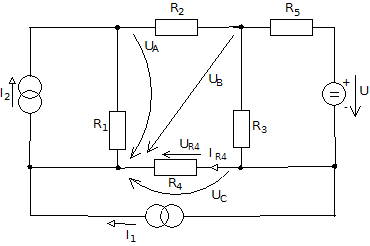
\includegraphics[height=5cm]{obrazky/pr3a}
\end{figure}

\begin{flushleft}
\textbf{Postup:} \\ 
1. Na základe 1. Kirchohofoveho zákona si zostavíme rovnice pre uzly A,B,C. \\
\end{flushleft}

\begin{align*}
&A: I_2-I_{R2}- I_{R1} = 0\\
&B: I_{R2}+I_{R5}-I_{R3} = 0\\
&C: I_{R3}-I_{R5}-I_{R4}-I_1 = 0\\
\end{align*}

\begin{flushleft}
Vyjadríme si rovnice pre jednotlivé prúdy v obvode.
\end{flushleft}

\begin{equation*}
I_{R1}*R_1 - U_A = 0 
\end{equation*}

\begin{equation*}
I_{R1} = \frac{U_A}{R_1} 
\end{equation*}

\begin{equation*}
I_{R2}*R_2 + U_B - U_A = 0 
\end{equation*}

\begin{equation*}
I_{R2} = \frac{U_A-U_B}{R_2}
\end{equation*}

\begin{equation*}
I_{R3}*R_3 + U_C - U_B = 0 
\end{equation*}

\begin{equation*}
I_{R3} = \frac{U_B-U_C}{R_3}
\end{equation*} 

\begin{equation*}
I_{R4}*R_4 - U_C = 0 
\end{equation*} 

\begin{equation*}
I_{R4} = \frac{U_C}{R_4}  
\end{equation*} 

\begin{equation*}
I_{R5}*R_5 - R_{R3}*R_3 - U = 0 
\end{equation*} 

\begin{equation*}
I_{R5} = \frac{U - U_B - U_C}{R_5} 
\end{equation*} 

\begin{flushleft}
Dosadíme do rovníc pre uzly A,B,C rovnice pre jednotlivé prúdy
\end{flushleft}

\begin{equation*}
A: I_2 -\frac{-U_A-U_B}{R_2}-\frac{U_A}{R_1} = 0  
\end{equation*} 

\begin{equation*}
B: \frac{U_A-U_B}{R_2}+\frac{U-U_B+U_C}{R_5}-\frac{U_B-U_C}{R_3} = 0  
\end{equation*} 

\begin{equation*}
C: \frac{U_B-U_C}{R_3}-\frac{U-U_B+U_C}{R_5}-\frac{U_C}{R_4} - I_1 = 0   
\end{equation*} 

\begin{flushleft}
Po dosadení hodnôt zo zadania a úprave rovníc dostaneme rovnice:
\end{flushleft}

\begin{equation*}
A: -75U_A+44U_B = -1023  
\end{equation*} 

\begin{equation*}
B: 1680U_A-4346U_B + 2666U_C = -190960  
\end{equation*} 

\begin{equation*}
C: 1720U_B-3400U_C = 151760
\end{equation*} 

\begin{flushleft}
Vznikla sústava rovníc, ktorú vyriešime pomocou Cramerovho pravidla (Determinanty určíme na základe Sarrussovho pravidla) : 
\end{flushleft}
 
$$
\begin{pmatrix}
-75 & 44 & 0 \\
1680 & -4346 & 2666 \\
0 & 1720 & -3400 \\
\end{pmatrix}
$$

\begin{center}
$D = (-75)*(-4346)*(-3400)+1680*1720*0+0*44*2666-(0)*(-4346)*0-2666*1720*(-75)-3400*44*1680$ \\
D = -512988000\\
Rovnako postupujeme aj pri zvyšných maticiach
\end{center}
 
$$
\begin{pmatrix}
-1023 & 44 & 0 \\
-190960 & -4346 & 2666 \\
151760 & 1720 & -3400 \\
\end{pmatrix}
$$

\begin{center}
$D_1$ = -21190831200
\end{center}
 
$$
\begin{pmatrix}
-75 & -1023 & 0 \\
1680 & -190960 & 2666 \\
0 & 151760 & -3400 \\
\end{pmatrix}
$$

\begin{center}
$D_2$ = -24193764000
\end{center}
 
$$
\begin{pmatrix}
-75 & 44 & -103 \\
1680 & -4346 & -190960 \\
0 & 1720 & 151760 \\
\end{pmatrix}
$$

\begin{center}
$D_3$ = 106581720000
\end{center}

\begin{equation*}
U_A = \frac{D_1}{D} = 41,3086 V
\end{equation*} 

\begin{equation*}
U_B = \frac{D_2}{D} = 47,1624 V
\end{equation*} 

\begin{equation*}
U_C = \frac{D_3}{D} = 20,7766 V
\end{equation*} 

\begin{equation*}
U_{R4} = U_C = 20,7766 V
\end{equation*} 

\begin{equation*}
I_{R4} = \frac{U_{R4}}{R_4} = 1.0389 A
\end{equation*} 


% End 3rd 
% --------------
% Start 4th

\newpage
\begin{flushleft}
\textbf{4. príklad}\\
Varianta: C
\end{flushleft}

\begin{tabular}{|c|c|c|c|c|c|c|c|c|c|}
\hline $U_1$ & $U_2$ & $R_1$ & $R_2$ & $R_3$ & $L_1$ & $L_2$ & $C_1$ & $C_2$  & $f$ \\ 
\hline
$35V$ & $45V$ & $10\Omega$ & $13\Omega$ & $11\Omega$ & $220mH$ & $70mH$ & $230\mu F$ & $85\mu F$ & $75Hz$ \\ 
\hline
\end{tabular}
\bigskip

\begin{flushleft}
\textbf{Zadanie:}\\
Pro napájecí napětí platí: $\mu_1 = U_1 * \sin (2\pi\omega ft)$. $\mu_2 = U_2 * \sin (2\pi\omega ft)$. Ve vztahu pro napětí $u_{C1} = U_{C_1} * \sin (2\pi ft + \varphi_{C_1})$ určete $|U_{C_1}|$ a $\varphi_{C_1}$. Použijte metódu smyčkových proudů.\\
Pozn: Pomocné "směry šipek napájacích zdrojů platí pre speciální časový okamžik $(t = \frac{\pi}{2\omega})$.""

\end{flushleft}
\bigskip



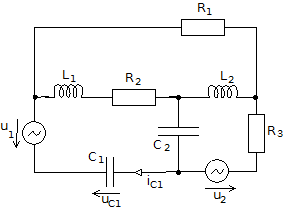
\includegraphics[height=6cm]{obrazky/pr4a}
\begin{flushleft}
Vytvoríme rovnice pro smyčkové proudy: \\
Napíšeme rovnice:
\end{flushleft}

\begin{equation*}
I_A: R_1*I_A + j\omega L_2(I_A-I_C)+R_2(I_A-I_B)+L_1(I_A-I_B)=0
\end{equation*}

\begin{equation*}
I_B: L_1*j\omega (I_B-I_A)+R_2(I_B-I_A)-j\frac{1}{\omega C_2}(I_B-I_C)-j\frac{1}{\omega C_1}I_B-U_1 = 0
\end{equation*}

\begin{equation*}
I_C: L_2*j\omega (I_C-I_A)+R_3*I_C - U_2 -j\frac{1}{\omega C_2}(I_C-I_B) = 0
\end{equation*}

\begin{flushleft}
Vypočítame $\omega$
\end{flushleft}

\begin{equation*}
\omega =2\pi f=2\pi 75 = 471,238898 rad/s
\end{equation*}

\begin{flushleft}
Upravíme rovnice:
\end{flushleft}

\begin{equation*}
I_A(R_1 + j\omega L_2 + R_2 +j\omega L_1) + I_B(-R_2-L_1j\omega ) + I_C(-j\omega L_2)=0
\end{equation*}

\begin{equation*}
I_A(-j\omega L_1 - R_2) + I_B(L_1j\omega+R_2-j\frac{1}{\omega C_2}-j\frac{1}{\omega C_1}) + I_C(j\frac{1}{\omega C_2})=U_1
\end{equation*}

\begin{equation*}
I_A(-j\omega L_2) + I_B(j\frac{1}{\omega C_2}) + I_C(j\omega L_2 +R_3-j\frac{1}{\omega C_2})=U_2
\end{equation*}

\newpage
\begin{flushleft}
Dosadíme hodnoty do rovníc a upravíme:
\end{flushleft}

\begin{equation*}
I_A(23+136,65925j) + I_B(-13-103,67255j) + I_C(-j32,9867)=0
\end{equation*}

\begin{equation*}
I_A(-13+103,67255j) + I_B(13+69,48069j) + I_C(j24,96548)=35
\end{equation*}

\begin{equation*}
I_A(-32,9867j) + I_B(24,96548j) + I_C(11+8,02122j)=45
\end{equation*}

\begin{flushleft}
Vznikla sústava rovníc, ktorú vyriešime pomocou Cramerovho pravidla (Determinanty určíme na základe Sarrussovho pravidla) : 
\end{flushleft}
 
$$
\begin{pmatrix}
23+136,65925j & -13-103,67255j & -32,9867j \\
-13+103,67255j & 13+69,48069j & 24,96548j \\
-32,9867j & 24,96548j & 11+8,02122j \\
\end{pmatrix}
$$

\begin{center}
$D = (23+136,65925j)*(13+69,48069j)*(11+8,02122j)+(-13+103,67255)*(24,96548j)*(-32,9867j)+(-32,9867j)*(-13-103,67255j)*(24,96548j)-(-32,9867j)*(13+69,48069j)*(-32,9867j)-(24,96548j)*(24,96548j)*(23+136,65925j)-(11+8,02122j)*(-13-103,67255j)*(-13+103,67255j)$ \\
$D$ = 16832.6466+8587.5831j\\
Rovnako postupujeme aj pri zvyšných maticiach
\end{center}

$$
\begin{pmatrix}
0 & -13-103,67255j & -32,9867j \\
35 & 13+69,48069j & 24,96548j \\
45 & 24,96548j & 11+8,02122j \\
\end{pmatrix}
$$

\begin{center}
$D_1$ = 18056.5297+48256.0005j
\end{center}

$$
\begin{pmatrix}
23+136,65925j & 0 & -32,9867j \\
-13+103,67255j & 35 & 24,96548j \\
-32,9867j & 45 & 11+8,02122j \\
\end{pmatrix}
$$

\begin{center}
$D_2$ = 8210.8774+52528.8410j
\end{center}

$$
\begin{pmatrix}
23+136,65925j & -13-103,67255j & 0 \\
-13+103,67255j & 13+69,48069j & 35 \\
-32,9867j & 24,96548j & 45 \\
\end{pmatrix}
$$

\begin{center}
$D_3$ = 61945.0351+25473.0289j
\end{center}

\begin{equation*}
I_A = \frac{D_1}{D} = 2,011684 + 1,84050j
\end{equation*}

\begin{equation*}
I_B = \frac{D_2}{D} = 1,650327+2,27869j
\end{equation*}

\begin{equation*}
I_C = \frac{D_3}{D} = 3,5326382-0,28895j
\end{equation*}

\begin{flushleft}
Vypočítame $I_{C1}$ a $U_{C1}$:
\end{flushleft}

\begin{equation*}
    I_{c1} = I_B = 1,650327 + 2,27869j V    
\end{equation*}
\begin{equation*}
    U_{c1} = -j\frac{1}{\omega C_1}*i_{c1} = -9,2263735j * i_{c1} = 21,0244 - 15,2268j V
\end{equation*}

\begin{flushleft}
Vypočítame $|U_{c1}|$:
\end{flushleft}

\begin{equation*}
\surd((Re)^2 + (Im)^2)) = \surd((21,0244)^2 + (-15,2268)^2)) = 25,9592 V
\end{equation*}

\begin{flushleft}
Fázový posun: 
\end{flushleft}

\begin{equation*}
   \varphi_{c1} = arctan(\frac{Im}{Re}) = -35^{\circ}54^{\prime}
\end{equation*}


% End 4th 
% --------------
% Start 5th

\newpage
\begin{flushleft}
\textbf{5. príklad}\\
Varianta: H
\end{flushleft}

\begin{tabular}{|c|c|c|c|}
\hline $U$ & $L$ & $R$ & $i_L(0)$ \\ 
\hline
$5V$ & $50H$ & $40\Omega$ & $2A$ \\ 
\hline
\end{tabular}
\bigskip

\begin{flushleft}
\textbf{Zadanie:}\\
Sestavte diferenciální rovnici popisující chování obvodu na obrázku, dále ji upravte
dosazením hodnot parametrů. Vypočítejte analytické řešení $i_L = f(t)$. Provedte kontrolu 
výpočtu dosazením do sestavené direnciální rovnice.		
\end{flushleft}
\bigskip

\begin{figure}[!h]
  \centering
  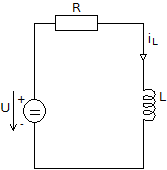
\includegraphics[height=5cm]{obrazky/pr5}
\end{figure}

\begin{flushleft}
Vyjadríme napätie na cievke $u_L$
\end{flushleft}

\begin{equation*}
   i_2*R +u_L-U=0
\end{equation*}

\begin{equation*}
   u_L = U -i_L*R
\end{equation*}

\begin{equation*}
   u_L=5-i_L*40
\end{equation*}

\begin{flushleft}
Vyjadríme vzťah pre diferenciálnu rovnicu a dosadíme doň napätie na cievke $u_L$
\end{flushleft}

\begin{equation*}
  i_L\prime =\frac{1}{L}(u_L)
\end{equation*}

\begin{equation*}
  i_L\prime =\frac{1}{50}(5-40*i_L)
\end{equation*}

\begin{equation*}
  i_L\prime =\frac{1}{10}-\frac{4}{5}i_L
\end{equation*}

\begin{equation*}
  i_L\prime + \frac{4}{5}i_L = \frac{1}{10}
\end{equation*}

\begin{flushleft}
Pre diferenciálnu rovnice vytvoríme očakávané riešenie
\end{flushleft}

\begin{equation*}
  i_L(t)=L(t)*e^{\lambda t}
\end{equation*}

\begin{flushleft}
Vypočítame lambdu: 
\end{flushleft}

\begin{equation*}
  \lambda + \frac{4}{5} = 0
\end{equation*}

\begin{equation*}
  \lambda = -\frac{4}{5} 
\end{equation*}

\begin{flushleft}
Dosadíme lambdu do očakávaného riešenia:  
\end{flushleft}

\begin{equation*}
  i_L(t)=L(t)*e^{-\frac{4}{5}t}
\end{equation*}

\begin{flushleft}
Vyjadríme hodnotu $i_L\prime $ a dosadíme do zostavenej diferenciálnej rovnice:  
\end{flushleft}

\begin{equation*}
  i_L\prime = L\prime (t)*e^{-\frac{4}{5}t} + L(t)*e^{-\frac{4}{5}t}(-\frac{4}{5})
\end{equation*}

\begin{equation*}
  L\prime (t)* e^{-\frac{4}{5}t} - (\frac{4}{5})L(t)*e^{-\frac{4}{5}t} + (\frac{4}{5})L(t)*e^{-\frac{4}{5}t} = \frac{1}{10}
\end{equation*}

\begin{equation*}
  L\prime (t)*e^{\frac{4}{5}t} = \frac{1}{10}
\end{equation*}

\begin{equation*}
  L\prime (t) = \frac{e^{\frac{4}{5}t}}{10}
\end{equation*}

\begin{equation*}
  \int L\prime (t)dt = \int \frac{e^{\frac{4}{5}t}}{10}dt
\end{equation*}

\begin{equation*}
  L(t) + k1 = \frac{5e^{\frac{4}{5}t}}{40} +k2
\end{equation*}

\begin{equation*}
  L(t) = \frac{e^{\frac{4}{5}t}}{8} + k
\end{equation*}

\begin{flushleft}
Dosadíme do očakávaného riešenia: 
\end{flushleft}

\begin{equation*}
  i_L(t) = L(t)*e^{\lambda t}
\end{equation*}

\begin{equation*}
  i_L(t) = (\frac{e^{\frac{4}{5}t}}{8} + k) *e^{-\frac{4}{5}t}
\end{equation*}

\begin{flushleft}
Získali sme obecné riešenie:  
\end{flushleft}

\begin{equation*}
  i_L(t) = \frac{1}{8} + k*e^{-\frac{4}{5}t}
\end{equation*}

\begin{flushleft}
Vypočítame k: 
\end{flushleft}

\begin{equation*}
  i_L(0) = \frac{1}{8} + k*e^{-\frac{4}{5}0}
\end{equation*}

\begin{equation*}
  2 = \frac{1}{8} + k
\end{equation*}

\begin{equation*}
  k = \frac{15}{8}
\end{equation*}

\begin{flushleft}
úplné riešenie získame dosadením k do obecného riešenia: 
\end{flushleft}

\begin{equation*}
  i_L(t) = \frac{1}{8} + \frac{15}{8}*e^{-\frac{4}{5}t}
\end{equation*}

\begin{flushleft}
Vykonáme kontrolu dosadením počiatočnej podmienky: 
\end{flushleft}

\begin{equation*}
  i_L(t) = \frac{1}{8} + \frac{15}{8}*e^{-\frac{4}{5}t}
\end{equation*}

\begin{equation*}
  i_L(0) = \frac{1}{8} + \frac{15}{8}
\end{equation*}

\begin{equation*}
  i_L(0) = 2A 
\end{equation*}

\begin{center}
Počiatočná podmienka platí.
\end{center}

\begin{flushleft}
Vykonáme kontrolu vyjadrením $i_L\prime$ a dosadením do diferenciálnej rovnice: 
\end{flushleft}

\begin{equation*}
  i_L(t) = \frac{1}{8} + \frac{15}{8}*e^{-\frac{4}{5}t}
\end{equation*}

\begin{equation*}
  i_L\prime (t) = -\frac{4}{5}\frac{15}{8}*e^{-\frac{4}{5}t}
\end{equation*}

\begin{flushleft}
Pôvodná diferenciálna rovnica:
\end{flushleft}

\begin{equation*}
  i_L\prime + \frac{4}{5}i_L = \frac{1}{10}
\end{equation*}

\begin{equation*}
  -\frac{4}{5}(\frac{15}{8}*e^{-\frac{4}{5}t}) + \frac{4}{5}(\frac{1}{8} + \frac{15}{8}*e^{-\frac{4}{5}t}) = \frac{1}{10}
\end{equation*}

\begin{equation*}
  \frac{4}{5}*\frac{1}{8} = \frac{1}{10}
\end{equation*}

\begin{equation*}
  \frac{1}{10} = \frac{1}{10}
\end{equation*}

\begin{center}
Hodnoty sa rovnajú a kontrola je vykonaná.
\end{center}

% end 5th
% ---
% Vysledky

\newpage
\begin{flushleft}
\textbf{Tabuľka výsledkov}
\end{flushleft}

\bigskip

\begin{tabular}{|c|c|l|}
\hline
Príklad & Zadanie & Výsledok \\ \hline
1 & C & $U_{R_8}$ = 15,5895V \hspace{5mm} $I_{R_8}$ = 0,0866A \\ \hline
2 & H & $U_{R_4}$ = 28,224V \hspace{5mm} $I_{R_4}$ = 0,0504A \\ \hline
3 & C & $U_{R_4}$ = 20,7766V \hspace{2mm} $I_{R_4}$ = 1.0389A \\ \hline
4 & C & $|U_{C_1}|$ = 25,9592V  \hspace{4mm} $\varphi_{C_1}$ = $-35^{\circ}54^{\prime}$ \\ \hline
5 & H & $i_L(t) = \frac{1}{8} + \frac{15}{8}*e^{-\frac{4}{5}t}$ \\ \hline
\end{tabular}



\end{document}